\documentclass{article}
\usepackage{amsmath}
\usepackage{enumerate}
\usepackage{fancyhdr} % Required for custom headers
\usepackage{lastpage} % Required to determine the last page for the footer
\usepackage{extramarks} % Required for headers and footers
\usepackage[usenames,dvipsnames]{color} % Required for custom colors
\usepackage{graphicx} % Required to insert images
\usepackage[tight,footnotesize]{subfigure} % Required for subfig
\usepackage{caption} % Required for subfig
\usepackage{hyperref} % Required for url
\usepackage{listings} % Required for insertion of code
\usepackage{courier} % Required for the courier font
\usepackage{lipsum} % Used for inserting dummy 'Lorem ipsum' text into the template
\topmargin=-0.45in
\evensidemargin=0in
\oddsidemargin=0in
\textwidth=6.5in
\textheight=9.0in
\headsep=0.25in
\linespread{1.1} % Line spacing
\pagestyle{fancy}
\lhead{\hmwkAuthorName} % Top left header
% \chead{\hmwkClass\ (\hmwkClassInstructor\ \hmwkClassTime): \hmwkTitle} % Top center head
\chead{\hmwkClass\ : \hmwkTitle} % Top center head
\rhead{\firstxmark} % Top right header
\lfoot{\lastxmark} % Bottom left footer
\cfoot{} % Bottom center footer
\rfoot{Page\ \thepage\ of\ \protect\pageref{LastPage}} % Bottom right footer
\renewcommand\headrulewidth{0.4pt} % Size of the header rule
\renewcommand\footrulewidth{0.4pt} % Size of the footer rule
\setlength\parindent{0pt} % Removes all indentation from paragraphs

% Define floor and ceiling
\def\lc{\left\lceil}   
\def\rc{\right\rceil}
\def\lf{\left\lfloor}   
\def\rf{\right\rfloor}

% table
\usepackage[table,xcdraw]{xcolor}
\usepackage{floatrow}
\newfloatcommand{capbtabbox}{table}[][\FBwidth]

% draw tree
\usepackage{tikz, tikz-qtree}
\usetikzlibrary{arrows,snakes,backgrounds,patterns,matrix,shapes,fit,calc,positioning,trees}
\tikzset{main node/.style={circle,fill=blue!20,draw,minimum size=1cm,inner sep=0pt},}

% Set your language 
%\lstset{language=Java}
\definecolor{codegreen}{rgb}{0,0.6,0}
\definecolor{codegray}{rgb}{0.5,0.5,0.5}
\definecolor{codepurple}{rgb}{0.58,0,0.82}
\definecolor{backcolour}{rgb}{0.95,0.95,0.92}
 
\lstdefinestyle{mystyle}{
    backgroundcolor=\color{backcolour},   
    commentstyle=\color{codegreen},
    keywordstyle=\color{magenta},
    numberstyle=\tiny\color{codegray},
    stringstyle=\color{codepurple},
    basicstyle=\footnotesize,
    breakatwhitespace=false,         
    breaklines=true,                 
    captionpos=b,                    
    keepspaces=true,                 
    numbers=left,                    
    numbersep=8pt,                  
    showspaces=false,                
    showstringspaces=false,
    showtabs=false,                  
    tabsize=2
}
\lstset{style=mystyle}

% Header and footer for when a page split occurs within a problem environment
\newcommand{\enterProblemHeader}[1]{
\nobreak\extramarks{#1}{#1 continued on next page\ldots}\nobreak
\nobreak\extramarks{#1 (continued)}{#1 continued on next page\ldots}\nobreak
}

% Header and footer for when a page split occurs between problem environments
\newcommand{\exitProblemHeader}[1]{
\nobreak\extramarks{#1 (continued)}{#1 continued on next page\ldots}\nobreak
\nobreak\extramarks{#1}{}\nobreak
}

\setcounter{secnumdepth}{0} % Removes default section numbers
\newcounter{homeworkProblemCounter} % Creates a counter to keep track of the number of problems

\newcommand{\homeworkProblemName}{}
\newenvironment{homeworkProblem}[1][Problem \arabic{homeworkProblemCounter}]{ % Makes a new environment called homeworkProblem which takes 1 argument (custom name) but the default is "Problem #"
\stepcounter{homeworkProblemCounter} % Increase counter for number of problems
\renewcommand{\homeworkProblemName}{#1} % Assign \homeworkProblemName the name of the problem
\section{\homeworkProblemName} % Make a section in the document with the custom problem count
\enterProblemHeader{\homeworkProblemName} % Header and footer within the environment
}{
\exitProblemHeader{\homeworkProblemName} % Header and footer after the environment
}

\newcommand{\problemAnswer}[1]{ % Defines the problem answer command with the content as the only argument
\noindent\framebox[\columnwidth][c]{\begin{minipage}{0.98\columnwidth}#1\end{minipage}} % Makes the box around the problem answer and puts the content inside
}

\newcommand{\homeworkSectionName}{}
\newenvironment{homeworkSection}[1]{ % New environment for sections within homework problems, takes 1 argument - the name of the section
\renewcommand{\homeworkSectionName}{#1} % Assign \homeworkSectionName to the name of the section from the environment argument
\subsection{\homeworkSectionName} % Make a subsection with the custom name of the subsection
\enterProblemHeader{\homeworkProblemName\ [\homeworkSectionName]} % Header and footer within the environment
}{
\enterProblemHeader{\homeworkProblemName} % Header and footer after the environment
}

\newlength{\tabcont}

\newcommand{\tab}[1]{%
\settowidth{\tabcont}{#1}%
\ifthenelse{\lengthtest{\tabcont < .25\linewidth}}%
{\makebox[.25\linewidth][l]{#1}\ignorespaces}%
{\makebox[.5\linewidth][l]{\color{red} #1}\ignorespaces}%
}%
%----------------------------------------------------------------------------------------------
%	NAME AND CLASS SECTION
%----------------------------------------------------------------------------------------------

\newcommand{\hmwkTitle}{Homework\ $\omega$} % Assignment title
\newcommand{\hmwkDueDate}{Monday,\ January\ 1,\ 2012} % Due date
\newcommand{\hmwkClass}{Fundamental Algorithms} % Course/class
\newcommand{\hmwkClassTime}{} % Class/lecture time
\newcommand{\hmwkClassInstructor}{Prof. Joel Spencer} % Teacher/lecturer
\newcommand{\hmwkAuthorName}{Songxiao Zhang, N10224459, {\tt 72}} % Your name

%----------------------------------------------------------------------------------------------
%	TITLE PAGE
%----------------------------------------------------------------------------------------------

\title{
\textmd{\textbf{\hmwkClass:\ \hmwkTitle}}\\
}
\author{\textbf{\hmwkAuthorName}}

\begin{document}

\maketitle

%----------------------------------------------------------------------------------------------
%	PROBLEM 1
%----------------------------------------------------------------------------------------------
\begin{homeworkProblem}
What's interesting about Fibonacci sequence is for number $f_m$ and $f_n$ with index $m$ and $n$
in the sequence, 
$$gcd(f_m,f_n) = f_{gcd(m,n)}$$

$A = BQ + R$ and $D = GCD[A,B] = GCD[B,R]$ 

$d=\gcd(89,55)=\gcd(55,34)=\gcd(34,21)=\gcd(21,13)=\gcd(13,8)$ \\
$=\gcd(8,5)=\gcd(5,3)=\gcd(3,2)=\gcd(2,1)=1$ \\

Given $D=BX' + RY' = BX' + (A-BQ)Y' = AY' + B[X' - QY']$, 
$$ X=Y', \ Y=X'-QY'$$
$X=-21,Y=34$ with $89x+55y=1$ as shown in Table~\ref{tab:gcdxy} in Page~\pageref{tab:gcdxy}.

\begin{table}[h]
\begin{tabular}{lllllll}
\hline
\rowcolor[HTML]{EFEFEF} 
A  & B  & Q & R  & \cellcolor[HTML]{ECF4FF}D & \cellcolor[HTML]{ECF4FF}X & \cellcolor[HTML]{ECF4FF}Y \\ 
\hline
89 & 55 & 1 & 34 & 1                         & -21                       & 34                        \\
55 & 34 & 1 & 21 & 1                         & 13                        & -21                       \\
34 & 21 & 1 & 13 & 1                         & -8                        & 13                        \\
21 & 13 & 1 & 8  & 1                         & 5                         & -8                        \\
13 & 8  & 1 & 5  & 1                         & -3                        & 5                         \\
8  & 5  & 1 & 3  & 1                         & 2                         & -3                        \\
5  & 3  & 1 & 2  & 1                         & -1                        & 2                         \\
3  & 2  & 1 & 1  & 1                         & 1                         & -1                        \\
2  & 1  & 1 & 1  & 1                         & 0                         & 1                         \\
1  & 1  & 1 & 0  & 1                         & 1                         & 0                         \\
1  & 0  &   &    &                           &                           &                           \\ 
\hline
\caption{Find $\gcd(89,55)$ with {\tt Extended-Euclid(a,b)}}
\label{tab:gcdxy}
\end{tabular}
\end{table}
\end{homeworkProblem}

%----------------------------------------------------------------------------------------------
%	PROBLEM 2
%----------------------------------------------------------------------------------------------
\begin{homeworkProblem}
$\frac{211}{507} = 211 \times 507^{-1} = 211 \times (-357 \bmod 1000) 
= 211 \times (-357) \bmod 1000 = 673 \bmod 1000 $ \\
shown in Table~\ref{tab:Z1000} in Page~\pageref{tab:Z1000}.

\begin{table}[ht!]
\begin{tabular}{lllllll}
\hline
\rowcolor[HTML]{EFEFEF} 
A    & B   & Q  & R   & \cellcolor[HTML]{ECF4FF}D & \cellcolor[HTML]{ECF4FF}X & \cellcolor[HTML]{ECF4FF}Y \\
\hline
1000 & 507 & 1  & 493 & 1                         & 181                       & -357                      \\
507  & 493 & 1  & 14  & 1                         & -176                      & 181                       \\
493  & 14  & 35 & 3   & 1                         & 5                         & -176                      \\
14   & 3   & 4  & 2   & 1                         & -1                        & 5                         \\
3    & 2   & 1  & 1   & 1                         & 1                         & -1                        \\
2    & 1   & 1  & 1   & 1                         & 0                         & 1                         \\
1    & 1   & 1  & 0   & 1                         & 1                         & 0                         \\
1    & 0   &    &     &                           &                           &                           \\
\hline
\end{tabular}
\caption{Find $\frac{211}{507}$ in $Z_{1000}$.}
\label{tab:Z1000}
\end{table}

\end{homeworkProblem}

%----------------------------------------------------------------------------------------------
%	PROBLEM 3
%----------------------------------------------------------------------------------------------
\begin{homeworkProblem}
We can observe that $\gcd(103, 101)=1$ by $\gcd(103, 101)=\gcd(101, 2)=\gcd(2,1)=1$  \\
$x\equiv 34 \bmod{101}$, $x\equiv 59 \bmod{103}$ \\
CRT $x\equiv c \bmod{103 \times 101}$ \\
Set $x=101y+34$, $$ 101y+34=59 \ in \ Z_{103} $$ 
                 $$ 101y=25  \ in \ Z_{103} $$ 
                 $$ y=101^{-1} \times 25 \ in \ Z_{103}$$ 
                 shown in Table~\ref{tab:qsys} in Page~\pageref{tab:qsys}.
\begin{table}[h]
\begin{tabular}{lllllll}
\hline
\rowcolor[HTML]{EFEFEF} 
A   & B   & Q  & R & \cellcolor[HTML]{ECF4FF}D & \cellcolor[HTML]{ECF4FF}X & \cellcolor[HTML]{ECF4FF}Y \\ \hline
103 & 101 & 1  & 2 & 1                         & -50                       & 51                        \\
101 & 2   & 50 & 1 & 1                         & 1                         & -50                       \\
2   & 1   & 2  & 0 & 1                         & 0                         & 1                         \\
1   & 0   &    &   &                           &                           &                           \\
\hline
\end{tabular}
\caption{Solve the system $x\equiv 34 \bmod{101}$, $x\equiv 59 \bmod{103}$. }
\label{tab:qsys}
\end{table}

$x=101y+34 \\
= 101 \times (101^{-1} \times 25 \bmod 103) + 34 \\
= 101 \times (51 \times 25 \bmod 103) + 34 \\
= 101 \times (39 \bmod 103) + 34 \\
= 34 + 101 \times 39 \bmod 101 \times 103  \\
= 3973 \bmod 10403$    

\end{homeworkProblem}

%----------------------------------------------------------------------------------------------
%	PROBLEM 4
%----------------------------------------------------------------------------------------------
\begin{homeworkProblem}
We can reduce this problem by double factorization and induction on both 1000 and 1001, 
shown in Table~\ref{tab:IslandHopping} in Page~\pageref{tab:IslandHopping}.

Factorization on $1000$ on base $2$: 
    $$ 1000 = \sum^N 2^i, \ where \  i \in N=\{3, 5, 6, 7, 8, 9\} $$

\begin{table}[h]
\begin{tabular}{llllll}
\hline
\rowcolor[HTML]{EFEFEF} 
i & $2^i$ & $\lfloor \frac{1001}{2^i} \rfloor$ & 1001 - $\lfloor \frac{1001}{2^{i-1}} \rfloor$
& ${2^{2^{i-1} \bmod 1001}}$ & ${2^{2^{i-1} \bmod 1001}}  \bmod 1001$ \\ 
\hline
0 & 1   & 0 & 0    & 2      & 2   \\
1 & 2   & 0 & 0    & 4      & 4   \\
2 & 4   & 0 & 0    & 16     & 16  \\
3 & 8   & 1 & 1    & 256    & 256 \\
4 & 16  & 0 & 8    & 65536  & 471 \\
5 & 32  & 1 & 40   & 221841 & 620 \\
6 & 64  & 1 & 104  & 16     & 16  \\
7 & 128 & 1 & 232  & 256    & 256 \\
8 & 256 & 1 & 488  & 65536  & 471 \\
9 & 512 & 1 & 1000 & 65536  & 620 \\
\hline
\end{tabular}
\caption{Using the Island-Hopping Method to find $2^{1000}$ modulo $1001$}
\label{tab:IslandHopping}
\end{table}

Then we can inductively calculate the result by only handling numbers under 1001 by 
$2^{2^i} \bmod 1001$. Calculator surely can handle any number below $2^6$. 

$$2^{1000} \bmod 1001 = \prod^N 2^{2^i} \bmod 1001, \ where \ i \in N=\{3, 5, 6, 7, 8, 9\} $$
$2^{1000} \bmod 1001 = (256 \times 620 \times 16 \times 256 \times 471 \times 620) \bmod 1001 = 562 \bmod 1001$.
(during each step, do $\bmod 1001$)

\end{homeworkProblem}

%----------------------------------------------------------------------------------------------
%	PROBLEM 5
%----------------------------------------------------------------------------------------------
\begin{homeworkProblem}
$\pi[v]=v$ means $v$ is the root of a tree with $37$ vertices, including $v$. And it's so far 
the largest tree in the forest. \\

$\pi[v]=u\neq v$ means there's a larger tree that rooted at $u$ with $SIZE[u] > 37$. 
And the tree that rooted at $v$ with $37$ vertices would be added to the tree that rooted at $u$
by a branch $(v, i)$ where $i$ is in the tree that rooted at $u$. \\

$w$ can have 2 values, either itself if it's always the root, or another vertex (was a root) 
in the tree when it was added to the root of a larger tree sometime. \\

$1 \leq $ the number of possible values of $SIZE[w] \leq V$. 
\end{homeworkProblem}

% \begin{lstlisting}[frame=single]
% \end{lstlisting}

% \begin{enumerate}[a.]
%     \item 
        %   
% \end{enumerate}

% \begin{figure}[h!]
%     \centering
%     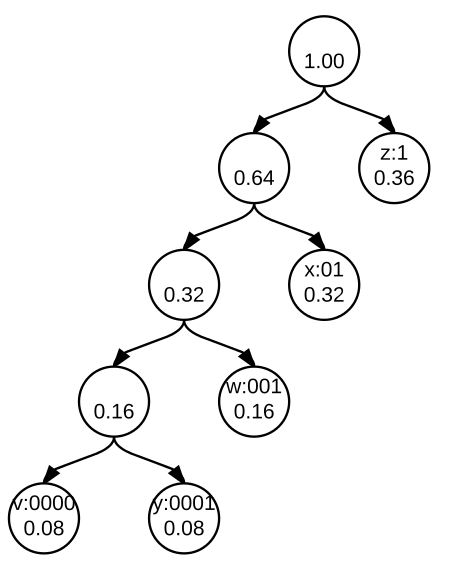
\includegraphics[scale=0.4]{hw8/2.png}
%     \caption{}
%     \label{fig:forz}
% \end{figure} 

% Figure~\ref{fig:tree} on Page~\pageref{fig:tree}.
% \begin{figure}[h!]
%     \centering
%     \subfigure[]{\label{}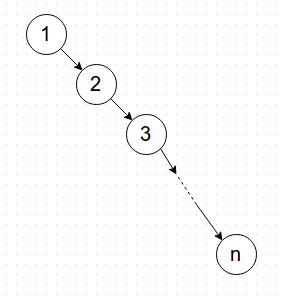
\includegraphics[scale=0.4]{hw6/51.png}}
%     \subfigure[]{\label{}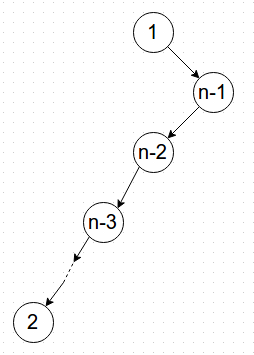
\includegraphics[scale=0.4]{hw6/52.png}}
%     \caption{}
%     \label{fig:tree}
% \end{figure} 

% \begin{tikzpicture}
%   [scale=.6,auto=left,every node/.style={circle,fill=blue!20}]
%   \node (n1) at (6, 6) {1};
%   \node (n2) at (4,3)  {2};
%   \node (n3) at (2,0) {3};
%   \foreach \from/\to in {n1/n2,n2/n3}
%     \draw (\from) -- (\to);
% \end{tikzpicture}

% \begin{tikzpicture}[
% >=stealth', semithick, node distance=1cm, level distance=15mm, 
%     level/.style={sibling distance=30mm/#1},
%     round/.style = {draw, circle, fill=blue!20, scale=0.8,minimum height=1cm},
%     every node/.style={circle, draw, fill=none, anchor=north},
% ]
% \node (tree 1) [draw=none, rectangle] {\tikz{%
% \node (tree 1) [round] {Q(1,16)}
%     child{ node[round] {S(2,7)} }
% }};
% \node (tree 2) [draw=none, rectangle, right=of tree 1] {\tikz{%
% \node (tree 2) [round] {R(17,20)}
% }};
% \end{tikzpicture}

\end{document}